\documentclass[12pt]{article}
\author{Lawrence Liu}
\usepackage{subcaption}
\usepackage{graphicx}
\usepackage{amsmath}
\usepackage{pdfpages}
\newcommand{\Laplace}{\mathscr{L}}
\setlength{\parskip}{\baselineskip}%
\setlength{\parindent}{0pt}%
\usepackage{xcolor}
\usepackage{listings}
\definecolor{backcolour}{rgb}{0.95,0.95,0.92}
\usepackage{amssymb}
\lstdefinestyle{mystyle}{
    backgroundcolor=\color{backcolour}}
\lstset{style=mystyle}

%\documentclass[12pt]{article}
%\title{ECE C143A Homework 6}
%\usepackage{subcaption}
%\author{Lawrence Liu}
%\usepackage{graphicx}
%\usepackage{amsmath}
%\usepackage{pdfpages}
%\newcommand{\Laplace}{\mathscr{L}}
%\setlength{\parskip}{\baselineskip}%
%\setlength{\parindent}{0pt}%
%\usepackage{xcolor}
%\usepackage{listings}
%\definecolor{backcolour}{rgb}{0.95,0.95,0.92}
%\usepackage{amssymb}
%\lstdefinestyle{mystyle}{
%    backgroundcolor=\color{backcolour}}
%\lstset{style=mystyle}
\title{ECE 231A HW 1}
\begin{document}
\maketitle
\section*{Problem 1}
If there was no slackness in the Kraft Inequality, then we would have 
$$\sum_{i=1}^m D^{l_m-l_i}<D^{l_m}$$
For the max length $l_m$. This means that for some nodes on level $l_m$ that is not a descendent of a codeword, or a codeword. Therefore while this node would be uniquely decodable but not able to form a sentence.
\section*{Problem 2}
Since a uniquely decodable code is a instantanous code we can use 
the Kraft Inequality. We have
$$\sum_{i=1}^{6}D^{-l_i}\leq1$$
The smallest D that satisfies this is $D=3$, therefore a good
lower bound on $D$ would be $\boxed{3}$.
\section*{Problem 3}
\subsection*{(a)}
The entropy of $H(X)$ is
$$H(X)=-\sum_{x\in X} p(x)\log_2\left(p(x)\right)$$
and we have that
\begin{align*}
	H(X|Y)&=\sum_{x\in X, y \in Y} p(y)H(X|Y=y)\\
	&=\left(\sum_{x\in S}p(x)\right)H(X|Y=1)+\left(\sum_{x\notin S}p(x)\right)H(X|Y=0)
\end{align*}
We have
\begin{align*}
	H(X|Y=1)&=-\sum_{x\in S}p(x|Y=1)\log_2(p(x|Y=1))\\
	&=-\sum_{x\in S}\frac{p(x)}{\sum_{x\in S}p(x)}\log_2\left(\frac{p(x)}{\sum_{x\in S}p(x)}\right)
\end{align*}
likewise we have
\begin{align*}
	H(X|Y=0)&=-\sum_{x\notin S}p(x|Y=0)\log_2(p(x|Y=0))\\
	&=-\sum_{x\notin S}\frac{p(x)}{\sum_{x\notin S}p(x)}\log_2\left(\frac{p(x)}{\sum_{x\notin S}p(x)}\right)
\end{align*}
Therefore we have
\begin{align*}
	H(X|Y)&=-\sum_{x\in S}p(x)\left(\log_2(p(x))-\log_2\left(
		\sum_{x\in S}p(x)
	\right)\right)-\sum_{x\notin S}p(x)\left(\log_2(p(x))-\log_2\left(
		\sum_{x\notin S}p(x)
	\right)\right)\\
	&=H(X)+\sum_{x\in S}p(x)\log_2\left(
		\sum_{x\in S}p(x)
	\right)+\sum_{x\notin S}p(x)\log_2\left(
		\sum_{x\notin S}p(x)
	\right)
\end{align*}
Therefore we have
$$H(X)-H(X|Y)=-\sum_{x\in S}p(x)\log_2\left(
	\sum_{x\in S}p(x)
\right)-\sum_{x\notin S}p(x)\log_2\left(
	\sum_{x\notin S}p(x)
\right)$$$$H(X)-H(X|Y)=\boxed{-q\log_2(q)-(1-q)\log_2(1-q)}$$
\subsection*{(b)}
$H(X)-H(X|Y)$ is maximized when 
$\sum_{x\in S}p(x)=\sum_{x\notin S}p(x)=\frac{1}{2}$, this is possible
when $S=\boxed{2,5}$ or $S=\boxed{1,2,4}$
\subsection*{(d)}
I would use Huffman Coding, and ask the questions in the following format,\\
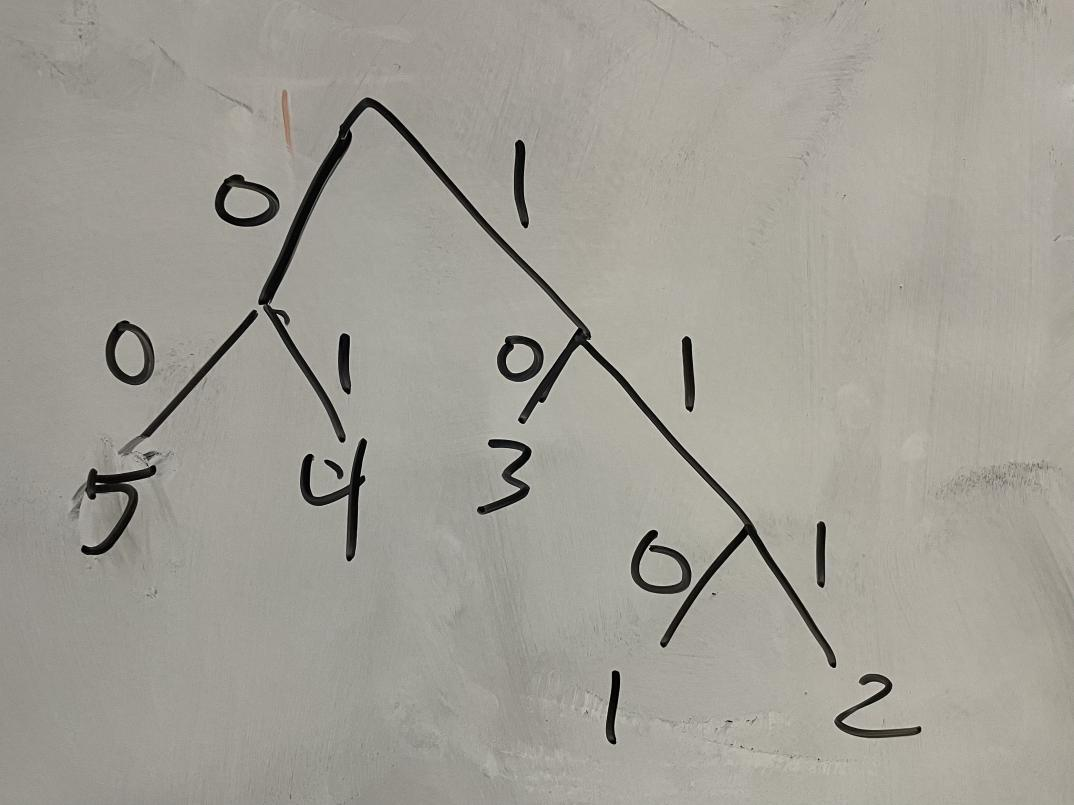
\includegraphics[scale=0.25]{fig0.jpg}\\
the average question length would be $\boxed{2.25}$
\section*{Problem 4}
\subsection*{(a)}
If a codeword is $l_j$ long, but if it has to start with $C(i)$, then it would be effectively be
concatenating $C(i)$ with a code word from $A_{j-i}$, ie all the code words with length $l_j-l_i$. Therefore the total number of words 
of $A_j$ would be the total combinations of $A_{j-i}$, ie $2^{l_j-l_i}$\\\\
Likewise, if a codeword is $l_j$ long, but if it has to end with $C(i)$, then it would be effectively be
concatenating a code word from $A_{j-i}$ with $C(i)$, ie all the code words with length $l_j-l_i$. Therefore the total number of words 
of $A_j$ would be the total combinations of $A_{j-i}$, ie $2^{l_j-l_i}$
\subsection*{(b)}
If we assume that $l_j>l_i$ we would have that the total number of words to remove from $A_j$ would
be the toal number of words to remove that start with $C(i)$ plus the total number of words that end with
$C(i)$. Therefore we would have that the total number of words to remove would be $2^{l_j-l_i+1}$. 
And if $l_j=l_i$ then we would only remove $1$ word, $C(i)$.
\subsection*{(c)}
We have that for any $1\leq j\leq k$, in order for the algorithm to not fail, we must
have that the number of inital codewords, is greater than the number
of removed code words, in otherwords we must have that
$$2^{l_j}>\sum_{i=1}^{j-1}2^{l_j-l_i+1}$$
Since, $\sum_{i=1}^{j-1}2^{l_j-l_i+1}<\sum_{i=1}^{j}2^{l_j-l_i+1}$, we can
assure the above inequality will be satisfied by the following inequality:
$$2^{l_j}\geq\sum_{i=1}^j2^{l_j-l_i+1}$$
This can be generalized to 
$$2^{l_k}\geq\sum_{i=1}^k2^{l_k-l_i+1}$$
Since for $1\leq j \leq k$:
\begin{align*}
	2^{l_k}&\geq\sum_{i=1}^k2^{l_k-l_i+1}\\
	2^{l_k}2^{l_j-l_k}&\geq2^{l_j-l_k}\sum_{i=1}^k2^{l_k-l_i+1}\\
	2^{l_j}&\geq\sum_{i=1}^k2^{l_j-l_i+1}\geq \sum_{i=1}^j2^{l_j-l_i+1}
\end{align*}
Therefore we could rearange the inequality to 
$$1\geq\sum_{i=1}^j2^{-l_i+1}$$
$$\sum_{i=1}^j2^{-l_i+1}\leq\frac{1}{2}$$
\subsection*{(d)}
Let $E[length(C(U))]=L$, we want to minimize
$$L=\sum_{i=1}^k p_il_i$$
given
$$\sum_{i=1}^k 2^{-l_i}\leq\frac{1}{2}$$
Using a langrange multipler, we get
$$J=\sum_{i=1}^{k}p_il_i+\lambda\sum_{i=1}^k 2^{-l_i}$$
$$\frac{\partial J}{\partial l_i}=p_i-\lambda 2^{-l_i}\ln(2)$$
Therefore we get that
$$2^{-l_i}=\frac{p_i}{\lambda \ln(2)}$$
Plugging this into $\sum_{i=1}^{k}2^{-l_i}\leq\frac{1}{2}$, we get
$$\lambda=\frac{2}{\ln(2)}$$
Therefore we get that
$$2^{-l_i}=\frac{p_i}{2}$$
And thus the optimal code length is
$$l_i^*=-\log_2{p_i}+\log_2(2)$$
But since $l_i$ must be an integer we have
$$-\log_2(p_i)\leq l_i\leq-\log_2(p_i)+2$$
Therefore we have that
$$-\sum_{i=1}^k p_i\log_2(p_i)\leq \sum_{i=1}^k p_i l_i \leq \left(-\sum_{i=1}^k p_i\log_2(p_i)\right)+2$$
Or in other words:
$$H(U)\leq E[length(C(U))] \leq H(U)+2$$
\section*{Problem 5}
\subsection*{(a)}
We have that 
$$H(X)=-\sum_{i\in \chi_1}(1-\gamma)p(i)\log_2\left((1-\gamma)p(i)\right)-
\sum_{i\in \chi_2}\gamma q(i)\log_2\left(\gamma q(i)\right)$$
Likewise for $H(X,Y)$ we have
$$H(X,Y)=-\sum_{y \in \{1,2\}}\sum_{x\in\{1,2,..m\}}P(x,y)\log_2(P(x,y))$$
we have that
$$p(x,1)=\begin{cases}
	(1-\gamma)p(x) & \text{if } x\in \chi_1\\
	0 & \text{if } x\notin \chi_2
\end{cases}$$
$$p(x,2)=\begin{cases}
	0 & \text{if } x\in \chi_1\\
	\gamma q(x) & \text{if } x\notin \chi_2
\end{cases}$$
Therefore we have
$$H(X,Y)=-\sum_{i\in \chi_1}(1-\gamma)p(i)\log_2\left((1-\gamma)p(i)\right)-
\sum_{i\in \chi_2}\gamma q(i)\log_2\left(\gamma q(i)\right)$$
And thus we have 
$$\boxed{H(X,Y)=H(X)}$$
\subsection*{(b)}
\begin{align*}
	H(X)&=-\sum_{i\in \chi_1}(1-\gamma)p(i)\log_2\left((1-\gamma)p(i)\right)-
\sum_{i\in \chi_2}\gamma q(i)\log_2\left(\gamma q(i)\right)\\
&=-(1-\gamma)\sum_{i\in \chi_1}p(i)\left(\log_2(p(i))+\log_2(1-\gamma)\right)-\gamma \sum_{i\in \chi_2}q(i)\left(\log_2(q(i))+\log_2(\gamma)\right)\\
&=-(1-\gamma)\left(\log_2(1-\gamma)+\sum_{i\in \chi_1}p(i)\log_2(p(i))\right)-\gamma\left(\log_2(\gamma)+\sum_{i\in \chi_2}q(i)\log_2(q(i))\right)\\
&=-(1-\gamma)\left(\log_2(1-\gamma)-H(X_1)\right)-\gamma\left(\log_2(\gamma)-H(X_2)\right)\\
&=\boxed{(1-\gamma)\left(H(X_1)-\log_2(1-\gamma)\right)+\gamma\left(H(X_2)-\log_2(\gamma)\right)}
\end{align*}
\subsection*{(c)}
Assuming $H(X_1)$ and $H(X_2)$ are in units of shannons we have, that to maximize $H(x)$ with take the derivative of $H(X)$ with respect to $\gamma$ we get
\begin{align*}
	\frac{\partial H(X)}{\partial \gamma}&=(\log_2(1-\gamma)-H(X_1))+(H(X_2)-\log_2(\gamma))
\end{align*}
This is maximized when 
\begin{align*}
	\frac{\partial H(X)}{\partial \gamma}&=0\\
	(\log_2(1-\gamma)-H(X_1))+(H(X_2)-\log_2(\gamma))&=0\\
	H(X_2)-H(X_1)&=\log_2(\gamma)-\log_2(1-\gamma)\\
	e^{H(X_2)-H(X_1)}&=\frac{\gamma}{1-\gamma}\\
	{1-\gamma}e^{H(X_2)-H(X_1)}&=\gamma\\
	\gamma&=\boxed{\frac{2^{H(X_2)-H(X_1)}}{1+2^{H(X_2)-H(X_1)}}}
\end{align*}


\section*{Problem 6}
\subsection*{(a)}
\begin{align*}1,2
	H(x)&=-\sum_{x\in X} p(x)\log_2(p(x))\\
	&=p(A)\log_2(p(A))+p(B)\log_2(p(B))+p(C)\log_2(p(C))\\&+p(D)\log_2(p(D))+p(E)\log_2(p(E))+p(F)\log_2(p(F))\\
	&=\frac{1}{2}\log_2(4)+\frac{1}{4}\log_2(8)+\frac{3}{16}\log_2(\frac{16}{3})+\frac{1}{16}\log_2(16)\\
	&=\boxed{2.452\text{ shannons}}
\end{align*}
\subsection*{(b)}
We have the following binary Huffman Encoding,\\
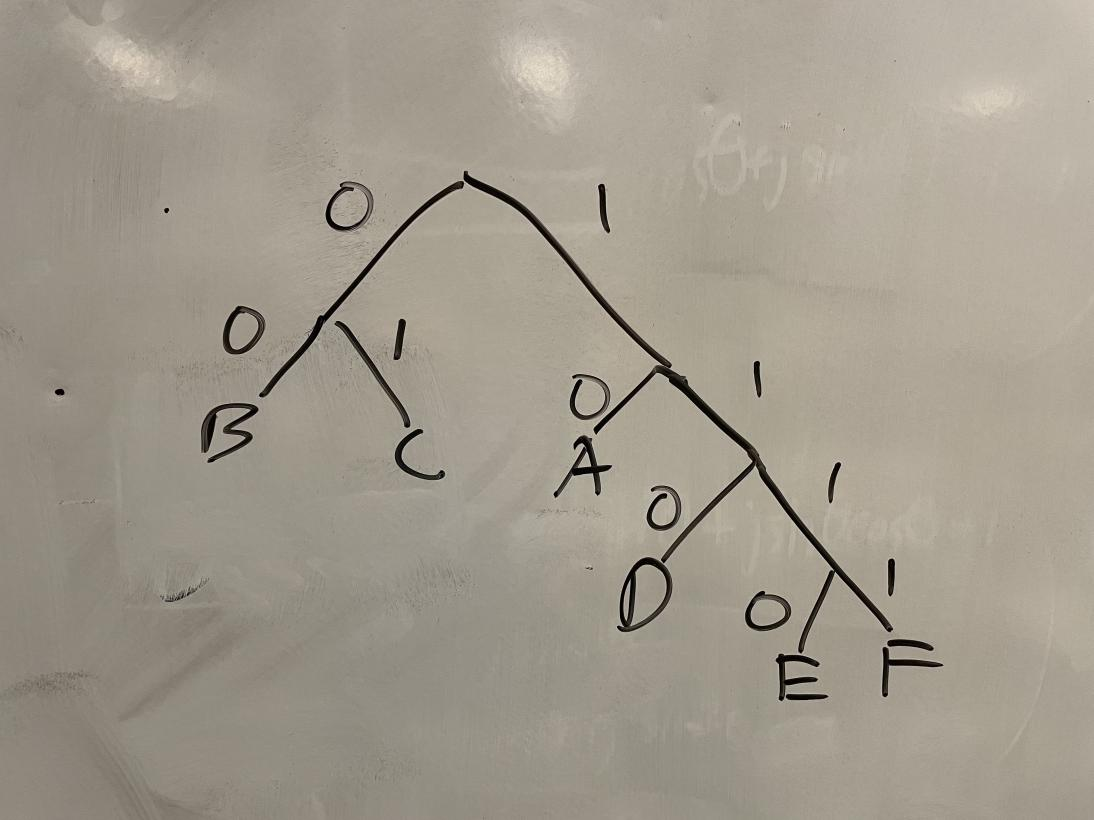
\includegraphics[scale=0.25]{fig1.jpg}\\

the expected length is $\boxed{2.5}$.
\end{document}
